
\iffalse
\begin{figure}
    \centering
    \includegraphics[width=12cm]{../figures/blip_bbh_runs_two_panel_comparison.pdf}
    \caption{Glitch panel comparison}
    \label{fig:qscan_null}
\end{figure}
\fi

\begin{table}[h!]
    \centering
    \renewcommand{\arraystretch}{1.2}
    \begin{tabular}{p{0.45\textwidth}|p{0.45\textwidth}}
    \toprule
    \textbf{LIGO-Virgo interferometers} & \textbf{Third-generation interferometers} \\
    \midrule
    \begin{enumerate}[leftmargin=*, label=\arabic*.]
        \item Detection rate of $\mathcal{O}(1)$ signal per week
        \item A GW signal is in-band for $\mathcal{O}(1)$ second to $\mathcal{O}(1)$ minute. Therefore, nearly every segment of data contains only noise. 
        \item Glitch rate of $\mathcal{O}(1)$ per minute across three observation runs. 
        \item \textit{Almost} all glitches occur in isolation due to smaller in-band duration and smaller detection rate of GW signals. 
        \item Almost all glitches can be vetoed without incurring significant loss of GW signals. 
    \end{enumerate}
    &
    \begin{enumerate}[leftmargin=*, label=\arabic*.]
        \item Detection rate of $\mathcal{O}(1)$ signal per minute
        \item A GW signal is in-band for $\mathcal{O}(1)$ minute to $\mathcal{O}(1)$ hour. Therefore, nearly every segment of data is expected to contain a signal. 
        \item Glitch rate is unknown. Let's assume same as LIGO-Virgo interferometers.
        \item \textit{Almost} all glitches will overlap with a GW signal due to larger in-band duration and larger detection rate. 
        \item Very few glitches may be vetoed without losing GW signals. 
    \end{enumerate}
    \\
    \bottomrule
    \end{tabular}
    \caption{Problem posed by glitches in LIGO-Virgo interferometers versus third-generation interferometers.}
    \label{tab:glitch_diff}
\end{table}
When occuring in the vicinity of a GW signal, glitches (or transient noises) can corrupt the signal. Such signal-overlapping glitches need to be carefully removed before analyzing the signal. From the 90 confident events detected across three observation runs by LIGO-Virgo interferometers, about 20 were contaminated by glitches and required some form of glitch mitigation~\cite{KAGRA:2021vkt}. This number will keep increasing as the interferometers collect more data. 

While glitch mitigation is an active area of research for current generation detectors, it is yet to recieve similar attention in the context of 3G-detectors. In Table~\ref{tab:glitch_diff}, we compare the problem posed by glitches for the LIGO-Virgo and the 3G interferometers. Glitches could turn out to be a major bottelneck in transitioning to the precision science era. In this chapter, we introduce the \texttt{nijntje} -- a null stream inspired noise transient elimination framework that is inexpensive, accurate, and scalable against the increasing computational cost of data analysis in 3G-era. Through \texttt{nijntje}, we demonstrate a clear edge that the null stream inherent in the triangular geometry of the Einstein Telescope provides for the precision science era. 

\section{The null stream}
By definition, a null stream is a linear combination of strain data from a network of GW detectors such that the signal (if present in the strain) cancels out. For the triangular geometry of the Einstein Telescope, the null stream can be constructed by summing the strain data from three interferometers. Let us denote the data from $i^{\mathrm{th}}$ interferometer by $\vec{d}_i$,
\begin{equation}
    \vec{d}_i = F_{+, i} \vec{h}_+ + F_{\times, i} \vec{h}_{\times},
\end{equation}
where $i$ varies from 1 to 3, $F_+$ and $F_{\times}$ are the antenna pattern functions, $h_+$ and $h_{\times}$ are the GW polarizations, defined in chapter~\ref{ch:gws}. The null stream is then given by
\begin{equation}
    \label{eq:null-stream-eq}
    \vec{d}_{\mathrm{null}} = \frac{1}{\sqrt{3}}\sum_{i = 1}^{3}\vec{d}_i,
\end{equation}
where the prefactor of $1/\sqrt{3}$ ensures that the noise’s power spectral density of null stream equals the average of those of the individual detectors. 

\begin{figure}
    \centering
    \includegraphics[width=\textwidth]{../figures/null_stream_antenna_pattern.pdf}
    \caption{Projection of plus (left) and cross (right) antenna pattern functions along the right ascension (RA) coordinate. Blue, red, and green lines show the antenna pattern functions of ET$_1$, ET$_2$, and ET$_3$ respectively. The black line, which is equal to zero for all values of RA, is obtained by summing the three. This feature gives rise to an inherent null stream in the triangular configuration of ET.}
    \label{fig:sum_patterns}
\end{figure}

The null stream is a geometic feature of the triangle configuration of ET. It comes about from the fact that the sum of antenna pattern function are individually zero, i.e.,
\begin{equation}
    \label{eq:sum_pattern}
    \sum_{i=1}^3 F_{+, i} = 0 ~ ~ \mathrm{and} ~ ~ \sum_{i=1}^3 F_{\times, i} = 0.
\end{equation}
Indeed, the individual antenna pattern functions vary over the whole sky and the equalities presented in Eq.~\eqref{eq:sum_pattern} hold for the whole sky as well. As an illustration, we show the projection of antenna pattern functions along the right ascension (RA) coordinate.

\section{A null-stream inspired noise transient elimination (\texttt{nijntje}) framework}
The \texttt{nijntje} framework uses the null stream of the triangular ET to remove signal-overlapping glitches. We demonstrate the workings of this framework using a toy model where a glitch is overlapping with a signal. We show how \texttt{nijntje} can effectively undo the effect of the glitch without corrupting the GW signal. Additionly, we also show how one can approach this problem without \texttt{nijntje} framework. 

We consider a toy model where a blip glitch is overlapping with a GW signal. 
\begin{figure}
    \centering
    \includegraphics[width=16cm]{../figures/assemble_nijntje.pdf}
    \caption{The blue box outlines the workflow of \texttt{nijntje} algorithm. \textit{Step 1}: Construct the null stream by summing the strain data from three interferometers. \textit{Step 2}: Using the null stream data and an RJMCMC method, perform an unmodelled reconstruction of the glitch timeseries. \textit{Step 3}: Find the glitch timeseries which corresponds to the median of the posterior samples and subtract it from $\mathrm{ET}_1$ frame. \textit{Step 4} (Optional): Perform parameter estimation using the cleaned data from $\mathrm{ET}_1$, and the existing data from $\mathrm{ET}_2$ and $\mathrm{ET}_3$ to verify the accuracy.}
    \label{fig:nijntje_chart}
\end{figure}

\section{Comparison between the triangle and L-shpaed interferometer}
\begin{figure}
    \centering
    \includegraphics[width=10cm]{../figures/et2l_delta_glitch_overlap_glitch_master.pdf}
    \caption{Glitch overlap}
    \label{fig:glitch_overlap}
\end{figure}

\begin{figure}
    \centering
    \includegraphics[width=10cm]{../figures/newsnr_mismatch_comparison.pdf}
    \caption{Mismatch}
    \label{fig:mismatch}
\end{figure}

\begin{figure}
    \centering
    \includegraphics[width=16cm]{../figures/newsnr_fig_4.pdf}
    \caption{Mass Distance Sky}
    \label{fig:delta_zero}
\end{figure}

\begin{figure}
    \centering
    \includegraphics[width=10cm]{../figures/newsnr_rank_10_single_block_percentile_parameters_short.pdf}
    \caption{Confidence interval}
    \label{fig:trend_delta}
\end{figure}
\section{Conclusions}
The null stream provides us with an extra piece of information~\ref{eq:null-stream-eq}. For the first time we show how we can use this infomation for precision science. 

\section{Caveats}


